\chapter{The X.509 standard and PKI}
We will now discuss the X.509 standard and Public Key Infrastructure 
(PKI), which is widelly adopted for public key certification.
\section{Public-key certificate (PKC)}
Lets begin with a definition:
\begin{boxH}
  A \textbf{public-key certificate} is a \textbf{data structure} to securely
  bind a public key to some attributes.
\end{boxH}
A PKC is said to "securely bind" a public key to some attributes
because it is signed by a trusted entity, the \textbf{Certification
Authority}, but other techniques for certification exists (e.g.
blockchain, direct trust and personal signature).\\
The attributes in the certificate are those employed in the
transaction being protected by the PKC, which are difficult to decide
a-priori without knowing the context: for example one attribute could
be an email address associated with the entity, which may not be valid
for all the transactions.\\
PKC are most important to achieve \textbf{non-repudiation}, many
certificates have legal value, and \textbf{digital signature} in a
secure way.\\
\begin{boxH}
  Keep in mind that a PKC is the complement of a corresponding
  \textbf{personal private key}, which is kept secret by the entity.
\end{boxH}
Which means that if the private key is compromised, the PKC is 
compromised as well.
\subsection{Key Generation in Public Key Cryptography (PKC)}

Key generation in public key cryptography (PKC) involves complex
algorithms and often relies on random number generators (RNGs) to
ensure strong, unpredictable keys. Once a key is generated, the
private key must be securely protected in various contexts:

\begin{itemize}
  \item \textbf{Storage}: The private key needs to be securely
    stored to prevent unauthorized access.
  \item \textbf{Usage}: The private key must also be protected when
    being used, as it could be exposed during operations in the CPU as
    it is used in clear text.
  \item \textbf{Software Application}: In software environments
    (e.g., web browsers), the trustworthiness of the computing
    platform must be considered, as it may be vulnerable to malware
    or weak implementations. This is true both for the context of
    key generation and use.
  \item \textbf{Dedicated Hardware}: Storing and using keys in
    dedicated hardware, such as a smart card, offers enhanced
    protection but comes with limitations in terms of algorithm
    updates or vulnerability patching( which may be difficult or
    even impossible). For example many old smart cards use 1024-bit 
    RSA keys, which are considered insecure today.
  \item \textbf{Key Injection}: Keys may be generated in software
    and injected into hardware devices, a process that can be useful
    for key recovery, but should be restricted to encryption keys to
    maintain security and ensure non repudiation. This is most
    important for the private key. 
\end{itemize}

PKC key management requires careful consideration of both security and
operational challenges, especially when dealing with long-term
security mechanisms.

\subsection{Certification architecture}

In Public Key Infrastructure (PKI), several key entities are
responsible for managing the lifecycle of Public Key Certificates
(PKCs):

\begin{itemize}
  \item \textbf{Certification Authority (CA)}: The CA is responsible
    for generating and revoking PKCs. It also publishes PKCs and
    maintains information about their status, such as whether they
    are valid or revoked, or even suspended.
  \item \textbf{Registration Authority (RA)}: The RA plays a
    critical role in verifying the claimed identity and attributes
    of a certificate requestor. It authorizes the issuance or
    revocation of PKCs but does not generate them itself.
  \item \textbf{Validation Authority (VA)}: The VA provides services
    that allow third parties to verify the validity status of a PKC,
    because some responsibilities or the RA may be delegated to it.
    This may involve downloading Certificate Revocation Lists (CRLs)
    or querying an Online Certificate Status Protocol (OCSP)
    responder to check the certificate's status in real-time.
  \item \textbf{Revocation Authority}: Although not an official
    term, this role may be assigned to either the RA or CA. The
    revocation authority is delegated to revoke certificates, often
    on a more urgent basis than their issuance (they are available
    most of the time), ensuring that compromised or invalid
    certificates are promptly rendered unusable.
\end{itemize}

These entities work together to ensure the security and
trustworthiness of PKC-based systems by handling key tasks such as
certificate issuance, verification, and revocation.

\subsection{Certificate generation}
The general
When an actor want to generate a certificate, it must first generate a 
key pair (public and private key). The private key is stored locally
and protected(encrypted) as good as possible, while the public key 
is sent to the CA with some attributes that help identify the actor.\\
The CA requires that the attributes are both correct and are
associated actually with the entity that is in control of the private
key, which requires authentication of the actor. For that purpose, if
the entity is a human it is usually required to go physically to the 
CA, even if in some cases a video call may be enough, with the 
requirement of showing a valid ID.\\
The Registration Authority will verify the attributes and the 
identity of the actor, and if everything is correct, it will send a 
message to the CA to generate the certificate.\\
At this point the CA generates the certificate, signs it with its 
private key and sends it back to the actor while also storing it in 
its repository.\\
As you may noticed, the verification is only on the attributes, and
not of the possession of the private key, which will be discussed
later.

\begin{figure}[h]
  \centering
  \includegraphics[width=0.8\textwidth]{img/x509 certificate
  generation.png}
  \caption{Certificate generation}
\end{figure}

\subsubsection{Another certificate generation architecture}

In addition to what just discussed, alternative architectures for
certificate generation exist:

\begin{itemize}
  \item \textbf{Key Pair Generation by RA}: In some architectures, the
    Registration Authority (RA) generates the key pair on behalf of
    the user, obtains the Public Key Certificate (PKC), and securely
    distributes the key pair and certificate to the user via a
    secure device, such as a smart card. This approach is often used
    in large companies where the employees are already known to the
    organization.

  \item \textbf{User Authentication via Code}: Another common method
    involves the user visiting the RA to obtain a code that can be
    used to authenticate their certificate request to the
    Certification Authority (CA). The code is typically calculated
    as a Message Authentication Code (MAC) using the shared secret
    key between the RA and CA:

    \[
      \text{code} = \text{MAC}(K, ID)
    \]

    where \(K\) is a shared secret key between the RA and CA, and
    \(ID\) is the user's identity. The user then submits this code to
    the CA to validate the certificate request.
\end{itemize}

These alternative methods provide flexibility for organizations with
different security needs, allowing for centralized key generation and
secure certificate distribution.

\section{X.509 certificates}

X.509 is an ITU-T (international telecommunication unit body) standard
that defines the format of public key certificates used to verify the
identity of a key owner in cryptographic systems. X509 was developed
as a certification technology to protect the x500 directory service,
and has undergone several versions:

\begin{itemize}
  \item \textbf{v1 (1988)}: The initial version of the standard.
  \item \textbf{v2 (1993)}: A minor update with small improvements.
  \item \textbf{v3 (1996)}: Added extensions and introduced version
    1 of the attribute certificate.
  \item \textbf{v3 (2001)}: Further enhancements, including version
    2 of the attribute certificate, which are not used anymore.
\end{itemize}

X.509 is part of the larger X.500 standard for directory services,
often referred to as "white pages," which are used for managing
information about entities in a structured way(directory services).
X.509 provides a solution to the problem of securely identifying the
owner of a cryptographic key.

The certificates and their structures are defined using \textbf{ASN.1}
(Abstract Syntax Notation One), a standard interface for defining data
structures exchanged in networking environments in a neutral and 
platform-independent way. 

\subsection{PKC Scope}
A Public Key Certificate (PKC) contains information that uniquely
associates a cryptographic key with an entity. This binding between
the key and the entity is ensured by a \textbf{Trusted Third Party
(TTP)}, typically referred to as a Certification Authority (CA), which
digitally signs each certificate to guarantee its authenticity.\\

The liability associated with a PKC may be restricted to specific
applications or purposes, as outlined in the CA's certification
policy. This policy defines the intended usage and limits the scope of
the certificate, ensuring it is applied within the proper legal and
technical contexts.

\subsection{Certificate Policy (CP) and Certification Practice
Statement (CPS)}

According to RFC-3647, "Internet X.509 Public Key Infrastructure
Certificate Policy and Certification Practices Framework," both the
Certificate Policy (CP) and Certification Practice Statement (CPS)
play key roles in defining the use and management of Public Key
Certificates (PKCs):

\begin{itemize}
  \item \textbf{Certificate Policy (CP)}: A CP is a named set of rules
    that defines the applicability of a PKC to a specific community
    or class of applications with common security requirements. It
    establishes the minimum requirements for the issuance and
    management of certificates and can be followed by multiple
    Certification Authorities (CAs). For example, a government CP
    may apply to all certification providers issuing certificates
    for official use.

  \item \textbf{Certification Practice Statement (CPS)}: A CPS outlines
    the specific practices that a CA follows when issuing PKCs.
    While a CP specifies the general rules, the CPS provides
    detailed implementation procedures. Each CA develops its own
    CPS, which is tailored to its operations and describes how it
    meets the requirements set forth in the CP.
\end{itemize}

\subsection{X.500 Directory Service}

The X.500 directory service was the first system to use X.509v1
certificates. It aimed to manage information about people and entities
in a network. However, this early setup had three big issues:

\begin{itemize}
  \item \textbf{No Guarantees on the CA's Quality}: There weren't
    clear rules or policies to ensure that Certification Authorities
    (CAs) were reliable or trustworthy. People just had to trust the
    CA, which caused concern over the security of the certificates.

  \item \textbf{Lack of a proper X.500 Infrastructure}: Even though
    certificates were supposed to be stored in X.500 directories, the
    infrastructure to do this was never fully implemented worldwide.
    This made it tough to access certificates when needed.

  \item \textbf{Hard to Establish Certification Paths}: It was
    difficult to connect two users with certificates issued by
    different CAs because the relationships between CAs weren’t
    well-defined. With each CA running its own domain, figuring out
    how to establish a secure connection between users from different
    domains was tricky.
\end{itemize}

These issues slowed down the adoption of X.500 and made it clear that
better systems were needed for managing certificates.

\subsubsection{Fixing X.509v1 Problems}

To solve these problems, X.509v1 was updated with a couple of key
changes:

\begin{itemize}
  \item \textbf{Move the semantics Outside the Certificate}: Instead of
    relying on the certificate itself to define its semantics, they
    decided to put that responsibility on the application or some
    external system. This approach was used in things like RFC-1422
    (PEM), where the application takes care of interpreting the
    certificate.

  \item \textbf{Make Certificates More Flexible}: The original X.509v1
    certificates were pretty limited: they only had an identifier and a
    key. With X.509v3, they added more fields and options to make
    certificates more flexible and useful for a variety of purposes.
    This allowed them to handle a wider range of security scenarios.
\end{itemize}

These updates helped fix the early issues and set the stage for
broader adoption of the improved X.509v3 certificates.

\subsection{RFC-1422}
RFC-1422 tried to fix some of the problems with the early X.500
systems by proposing a worldwide certification hierarchy. The plan was
to have one main CA at the top: the \textbf{IPRA} (Internet Policy
Registration Authority). This CA would be responsible for setting the
rules and policies for all other CAs in the system, ensuring that
everyone followed the same security practices.\\
Instead of directly issuing certificates to lower-level CAs, the IPRA
would issue certificates to \textbf{Policy Certification Authorities
(PCAs)}.\\
The IPRA oversaw the entire structure and laid out specific
roles for different types of Certification Authorities (CAs) to manage
and enforce certificate policies:

\begin{itemize}
  \item \textbf{Policy Certification Authority (PCA)}: PCAs were
    responsible for setting and enforcing the policies that governed
    how certificates were issued. They made sure that the CAs under
    them followed the right security practices.
  
  \item \textbf{Name Subordination}: CAs had to issue certificates
    within a defined part of the naming structure, ensuring a
    consistent and organized system. For example:
  \begin{itemize}
      \item \textbf{CA n.1}: C=IT (country-level CA for Italy)
      \item \textbf{CA n.2}: C=IT, O=Politecnico di Torino (CA for an
        organization within Italy)
  \end{itemize}
\end{itemize}


 However, this system wasn’t without flaws—it
was still based on geographic hierarchies, which didn’t always match
the needs of modern, global organizations.

The IPRA was established, and four PCAs were created under it. One of
these PCAs was designated as \textbf{high assurance}, meaning it had
to carry out stricter checks before issuing certificates. For
instance, BBN, a company heavily involved with the U.S. military,
might require things like fingerprints or even DNA tests to verify
identities.

In contrast, \textbf{mid-level assurance} certificates, like those
issued by universities such as MIT, required less rigorous
checks—maybe just showing a passport. MIT could even set up its own
subordinate CAs, like one for the Laboratory for Computer Science, to
handle its internal certificate needs.

What’s interesting is how different cultural practices shaped the
certification process. In the U.S., where people don’t generally carry
ID cards, \textbf{residential certification authorities} were used. If
you wanted to open a bank account, for example, you might have to show
an electricity bill to prove your address. While this seems strange in
countries with formal ID systems, in the U.S., it was a necessity.

Finally, there were \textbf{persona certificates}, which allowed for
anonymous certificates. These were for users who didn’t want to reveal
their identity but still needed secure communications. For example,
you could be “anonymous user number 95.” Even though no one knew who
you were, the security of your communication was still guaranteed.

\begin{figure}[h]
  \centering
  \includegraphics[width=0.8\textwidth]{img/x509 internet per
  hierarchy.png}

  \caption{Internet PEM hierarchy (RFC-1422)}
\end{figure}

Unfortunately, this system was a complete failure for several reasons:

\begin{itemize}
  \item The hierarchical structure severely limited flexibility, much
    like the issues we saw with X.500. For international companies,
    this rigid hierarchy simply didn't work.

  \item Name subordination imposed additional restrictions. You
    couldn't just assign any name—you had to follow the strict
    hierarchy, which wasn't always practical.

  \item The use of the PCA concept lacked flexibility, especially in
    commercial settings. Instead of automating the process, a human
    operator was needed to check if the requester was following the
    policy. This made the system cumbersome and inefficient for
    businesses.

  \item Lastly, the biggest issue was trust. Where would the IPRA be
    placed? Naturally, the U.S. wanted it, but other countries, like
    Russia, China, or even Japan, wanted control as well. No one
    trusted a single country to sit at the top of the hierarchy,
    fearing the possibility of a fake hierarchy being created. As a
    result, the experiment collapsed. It briefly existed, primarily
    used by the United States, but it never gained global traction.
\end{itemize}

\section{X.509 Version 3}

X.509 Version 3 is a standard that was finalized in June 1996 through
a collaborative effort between ISO, ITU, and the IETF, with the goal
of making certificates suitable for internet applications. This
version consolidated all the necessary updates to certificates and
Certificate Revocation Lists (CRLs) into a single document. Earlier
versions of X.509 (v1 and v2) relied on external semantics, such as
the failed attempt with the Internet PEM hierarchy, which proved
unsuccessful. X.509v3 addressed these shortcomings by ensuring
certificates would be useful for internet applications, particularly
as OSI applications became mostly obsolete.\\
Key features of X.509 Version 3 include:

\begin{itemize}
  \item \textbf{Types of Extensions}:
    \begin{itemize}
      \item \textbf{Public Extensions}: These are defined by the
        standard and made publicly available for anyone to use.
        Because they are standardized, any system or application
        should be able to understand and process them.
      \item \textbf{Private Extensions}: These are tailored to
        specific user communities and are not publicly available. If a
        system does not understand a private extension, it will treat
        it as a binary blob and discard it. Private extensions are
        crucial for certain organizations that require custom
        functionality.
    \end{itemize}
    
    The introduction of extensions is a major improvement in X.509v3,
    adding flexibility without changing the fundamental structure of
    the certificate (which remains the same as in X.509v1). Extensions
    are contained within a small field but open up a wide range of
    possibilities. Public extensions ensure standard compatibility,
    while private extensions allow customization specific to
    organizations.

  \item \textbf{Certificate Profile}: This refers to a set of
    extensions tailored for a specific purpose or application,
    ensuring that certificates meet particular requirements. For
    example, RFC 5280, titled "Internet X.509 Public Key
    Infrastructure Certificate and Certificate Revocation List (CRL)
    Profile," provides guidelines on how X.509 certificates and CRLs
    should be structured for protecting internet applications.
    Certificate profiles are important because they dictate how
    certificates should be used for different scenarios, ensuring
    consistency and security.
\end{itemize}


\subsection{Base syntax}

The base syntax of an X.509 certificate is defined as follows:

\begin{verbatim}
Certificate ::= SEQUENCE {
    signatureAlgorithm AlgorithmIdentifier,
    tbsCertificate TBSCertificate,
    signatureValue BIT STRING
}

TBSCertificate ::= SEQUENCE {
    version [0] Version DEFAULT v1,
    serialNumber CertificateSerialNumber,
    signature AlgorithmIdentifier,
    issuer Name,
    validity Validity,
    subject Name,
    subjectPublicKeyInfo SubjectPublicKeyInfo,
    issuerUniqueID [1] IMPLICIT UniqueIdentifier OPTIONAL,
        -- if present, version must be v2 or v3
    subjectUniqueID [2] IMPLICIT UniqueIdentifier OPTIONAL,
        -- if present, version must be v2 or v3
    extensions [3] Extensions OPTIONAL
        -- if present, version must be v3
}
\end{verbatim}

This abstract notation outlines the basic structure of the
certificate. The \texttt{Certificate} is defined as a sequence, which
is a data structure that includes several fields. The first field,
\texttt{signatureAlgorithm}, is the algorithm identifier used by the
Certificate Authority (CA) to sign the certificate. 

Next, the \texttt{tbsCertificate} (to be signed certificate) is of
type \texttt{TBSCertificate}, which contains the main information that
needs to be signed. Finally, the \texttt{signatureValue} is a bit
string that holds the actual signature.

The \texttt{TBSCertificate} is again defined as a sequence, starting
with the \texttt{version} field, which begins numbering with zero,
indicating version 1. For version 3, this field has a value of two.
Following that, we have the \texttt{serialNumber} of the certificate
and the \texttt{signature} algorithm identifier. 

You may wonder why the signature algorithm appears twice—once
externally and once within the \texttt{TBSCertificate}. The external
algorithm identifier is crucial for verifying the signature; without
knowing the algorithm, you cannot validate the signature value. Having
it specified internally helps ensure that the signature algorithm used
for verification matches the algorithm used for signing. If they
differ, it's a red flag, indicating that the certificate should not be
trusted.

The \texttt{issuer} field identifies the certification authority by
name, and the \texttt{validity} field specifies the validity period of
the certificate. The \texttt{subject} is identified by its name, and
the \texttt{subjectPublicKeyInfo} field contains both the algorithm
and the actual public key of the subject.

In addition, versions 2 and 3 introduce optional unique identifiers
for both the issuer and subject, though these identifiers are rarely
used today. Finally, the \texttt{extensions} field, which is optional,
must be present for certificates of version 3, as earlier versions do
not support extensions.


\subsection{Critical Extensions}

In the context of X.509 certificates, extensions can be classified as
critical or non-critical, each affecting the certificate verification
process differently:

\begin{itemize}
  \item \textbf{Critical Extensions}: If a certificate contains an
    unrecognized critical extension, it \textbf{MUST} be rejected
    during the verification process. This ensures that any essential
    information required for proper validation is recognized and
    handled appropriately.

  \item \textbf{Non-Critical Extensions}: Conversely, a non-critical
    extension \textbf{MAY} be ignored if it is unrecognized. This
    allows flexibility in certificate processing, as non-critical
    information does not impede the overall verification of the
    certificate.
\end{itemize}

The responsibility for handling these extensions lies entirely with
the entity performing the verification, referred to as the
\textbf{Relying Party (RP)}. The RP must implement logic to correctly
interpret and respond to both critical and non-critical extensions in
accordance with their definitions.

\subsection{Public Extensions}

X.509 version 3 defines four classes of public extensions that enhance
the functionality and applicability of certificates:

\begin{itemize}
  \item \textbf{Key and Policy Information}: Extensions in this
    class provide additional information regarding the key usage and
    policies applicable to the certificate, guiding how the key
    should be used within specific contexts.

  \item \textbf{Certificate Subject and Certificate Issuer
    Attributes}: These extensions include attributes related to both
    the subject of the certificate (the entity that the certificate
    represents) and the issuer (the Certification Authority),
    enabling more detailed identification and classification.

  \item \textbf{Certificate Path Constraints}: These extensions
    define rules and limitations regarding the certification path,
    ensuring that certificates can only be used in certain contexts
    or under specific conditions, enhancing security within the
    certificate hierarchy.

  \item \textbf{CRL Distribution Points}: This extension indicates
    where the Certificate Revocation List (CRL) can be found,
    providing necessary information for relying parties to check the
    revocation status of the certificate efficiently.
\end{itemize}

\subsection{Key and policy information}


There are six public extensions dedicated to this purpose. 
We won't discuss all of them, but we will focus on the most important 
ones.

\subsubsection{Authority Key Identifier}

Key and policy information extensions in X.509 v3 provide crucial
details about the public keys associated with certificates. One
significant component is the \textbf{Authority Key Identifier (AKI)},
which serves the following purposes:

\begin{itemize}
  \item \textbf{Identification of the Signing Key}: The AKI identifies
    a specific public key used to sign a certificate, ensuring that
    the verification process can accurately trace the certificate's
    authenticity back to the correct authority.

  \item \textbf{Identification Methods}: The identification can be
    achieved through:
    \begin{itemize}
      \item A \textbf{key identifier}, typically represented as the
        digest (hash) of the public key of the certification authority.
      \item The combination of \textbf{issuer-name} and 
        \textbf{serial-number}, allowing a clear reference to the
        issuing CA's key.
    \end{itemize}

  \item \textbf{Usage}: The AKI is particularly useful in scenarios
    where the same CA might utilize multiple keys, such as for 
    different assurance levels, like low assurance for general use 
    and high assurance for sensitive applications.

  \item \textbf{Non-Critical Extension}: While the AKI is classified 
    as non-critical, its presence can be vital in certain 
    applications. In the professor experience, the absence of this 
    extension can lead to many applications rejecting the certificate
    as invalid.

  \item \textbf{Importance in Certificate Chains}: When an 
    application receives a certificate, it often needs to establish 
    a trust path up to a root CA. This path-building process relies 
    heavily on the AKI field. If a CA neglects to include this 
    extension, it may lead to compatibility issues with various 
    applications, despite being non-critical.
\end{itemize}

\subsubsection{Subject key identifier}
The \textbf{Subject Key Identifier} (SKI) extension serves
to identify a specific public key associated with a certificate. Key
features include:

\begin{itemize}
  \item \textbf{Identification of Public Key}: The SKI uniquely
    identifies a particular public key used in an application. This
    is especially important in scenarios where the public key may be
    updated or replaced over time.

  \item \textbf{Being Non-Critical}: The SKI is classified as a
    non-critical extension, meaning that while it provides valuable
    identification information, its absence does not necessarily
    prevent the certificate from being considered valid.
\end{itemize}
This one is usually not present in the certificate because an
identifier is already present in the certificate.
\subsubsection{Key usage}

The \textbf{Key Usage} (KU) extension specifies the application
domains in which a public key may be utilized. Key characteristics
include:

\begin{itemize}
  \item \textbf{Application Domain Identification}: The KU extension
    identifies the specific purposes for which the associated public
    key can be employed, ensuring that it is used appropriately
    within defined contexts. In case of misuse, the application may
    refuse to accept the certificate and the CA may refuse liability.

  \item \textbf{Critical or Non-Critical}: The Key Usage extension
    can be classified as either critical or non-critical:
    \begin{itemize}
      \item If marked as \textbf{critical}, the certificate may only
        be used for the specific purposes indicated in the Key Usage
        extension. Any usage outside the defined scopes would render
        the certificate invalid.
      \item If marked as \textbf{non-critical}, the certificate can
        be used more flexibly, potentially allowing usage beyond the
        defined applications without invalidating the certificate.
    \end{itemize}

  \item \textbf{Permitted Cryptographic Operations}: The following
    cryptographic operations can be defined within the Key Usage
    extension:
    \begin{itemize}
      \item \textbf{digitalSignature}: valid in the certificate of a
        user but also in the certificate of a certification authority.
      \item \textbf{nonRepudiation}: Specifically permitted for
        users (non repudiation is only for humans after all).
      \item \textbf{keyEncipherment}: Permitted for users.
      \item \textbf{dataEncipherment}: Allowing encryption of data.
      \item \textbf{keyAgreement}: Involves:
        \begin{itemize}
          \item \textbf{encipherOnly}: Restricting use to
            enciphering operations.
          \item \textbf{decipherOnly}: Restricting use to
            deciphering operations.
        \end{itemize}
      \item \textbf{keyCertSign}: Specifically permitted for
        Certificate Authorities (CAs).
      \item \textbf{cRLSign}: Also permitted for Certificate
        Authorities (CAs) for signing Certificate Revocation Lists
        (CRLs).
    \end{itemize}
\end{itemize}

\subsubsection{Private key usage period}

The \textbf{Private Key Usage Period} extension in X.509 v3 specifies the
time frame during which the associated private key may be used. Key
features include:

\begin{itemize}
  \item \textbf{Usage Period Definition}: This extension defines the
    period during which the private key can be actively utilized,
    helping to enforce time-based restrictions on key usage.

  \item \textbf{Non-Critical Extension}: The Private Key Usage
    Period extension is always classified as non-critical, meaning
    that its absence does not invalidate the certificate. However,
    the information it provides can be important for managing key
    lifecycles.

  \item \textbf{Usage Discouraged}: While this extension is
    available, its use is generally discouraged in practice.
    Organizations often prefer to manage key lifetimes through other
    means, such as regular key rotation, rather than relying on a
    specified usage period within the certificate.
\end{itemize}

\subsubsection{Certificate policies}

The \textbf{Certificate Policies} extension outlines the specific
policies that were adhered to during the issuance of the certificate
and defines the purposes for which the certificate can be utilized.
Key aspects include:

\begin{itemize}
  \item \textbf{Policy Listing}: This extension provides a
    comprehensive list of the policies that govern the certificate
    issuance process, ensuring clarity regarding its intended use.

  \item \textbf{Indication Methods}: Certificate policies can be
    indicated using various formats, including:
    \begin{itemize}
      \item \textbf{Object Identifier (OID)}: A unique identifier for
        the policy.
      \item \textbf{Uniform Resource Identifier (URI)}: A link to a
        location where the policy can be reviewed.
      \item \textbf{Text Message}: A textual description of the
        policy.
    \end{itemize}

  \item \textbf{Critical or Non-Critical}: The Certificate Policies
    extension can be classified as either critical or non-critical:
    \begin{itemize}
      \item If marked as \textbf{critical}, the certificate must only
        be used in accordance with the specified policies; otherwise,
        it may be considered invalid.
      \item If marked as \textbf{non-critical}, the certificate can be
        used more flexibly, although the policies still provide
        guidance for its intended use.
    \end{itemize}

  \item \textbf{Support for Authentication and Authorization}: The use
    of this extension can enhance not only the authentication of users
    and entities but also facilitate authorization processes,
    providing a clearer understanding of the permissible actions
    associated with the certificate.
\end{itemize}

\subsubsection{Policy mappings}

The \textbf{Policy Mappings} extension in X.509 v3 establishes a
correspondence between policies across different certification
domains. Key aspects include:

\begin{itemize}
  \item \textbf{Mapping of Policies}: This extension indicates how
    policies from one certification authority (CA) correspond to
    policies from another, facilitating interoperability and trust
    among different certificate frameworks. This can be done
    automatically, but needs human interaction to be done correctly.

  \item \textbf{Presence in CA Certificates}: The Policy Mappings
    extension is typically present only in CA certificates, allowing
    certification authorities to define and communicate
    relationships between their policies and those of other
    authorities.

  \item \textbf{Non-Critical Extension}: The Policy Mappings
    extension is classified as non-critical, meaning its absence
    does not invalidate the certificate. However, it serves as an
    important tool for enhancing the understanding and usability of
    certificates across different domains.
\end{itemize}

\subsection{Certificate subject and issuer attributes}
As previously mentioned, the X.509 v3 standard includes extensions 
that provide additional information about the subject and issuer of a 
certificate. Without this extension, the only possible names are x500
ones, which aren't really an identifier.
\subsubsection{Subject Alternative Name (SAN)}
The Subject Alternative Name (SAN) extension provides a flexible way
to identify the owner of a certificate. This extension allows the use
of various formalisms to represent the owner, including e-mail
addresses, IP addresses, and URLs.\\
Importantly, the SAN field is always considered critical when the
subject name field is empty. This means that if there is no subject
name, the SAN extension must be present to ensure proper identification
and functionality of the certificate.

\subsubsection{Issuer Alternative Name (IAN)}
The Issuer Alternative Name (IAN) extension in enables the use of
various formalisms to identify the Certificate Authority (CA) that
issued a certificate or a Certificate Revocation List (CRL). This
extension supports different identifiers such as e-mail addresses, IP
addresses, and URLs.\\
The IAN field is always considered critical when the issuer name field 
is empty. In such cases, the IAN extension must be present to ensure 
proper identification of the issuing authority.\\

It's also interesting to see what are the possible identifiers that 
can be used in the IAN field.\\
 One option is the \textbf{RFC 802 Name}, which consists 
of the standard email addresses used in internet applications. The 
\textbf{DNS Name} identifies a node by its domain name, while an 
\textbf{IP Address} identifies the node by its numerical address. 
Another alternative is the \textbf{Uniform Resource Identifier (URI)}, 
which serves as an entry point on the web. This means that on the 
same node, you could have different certificates corresponding to 
various entry points for the applications.

In addition, you can use a \textbf{Directory Name}, which can be 
formatted according to X.500 or LDAP syntax. For example, the 
LDAP of the Politecnico di Torino might be represented as 
\texttt{country=T; organization=Politecnico di Torino; organizationUnit=Department}. 
While there is no formal management of country Italy in this case, 
the syntax remains consistent. 

Moreover, \textbf{X.400 Addresses} illustrate that these identifiers 
were still in use when version 3 was developed in 1996, as there 
were gateways that transformed mail from X.400 to RFC 802 formats. 
Thus, having the certificate associated with the X.400 address 
was essential. 

Next, we have the \textbf{EDI Party Name}, which stands for 
electronic data interchange. This standard allows companies to 
avoid manual processing of data. For instance, a car manufacturer 
might need to check if a supplier has specific tires available. 
Instead of making a phone call or sending a fax or email, they 
could use EDI to make a query through a neutral language that 
facilitates data requests and responses electronically. 

EDI serves as a general standard with various implementations, such 
as EDIFACT, which Stellantis and many other car manufacturers use 
to manage the availability of necessary items, check prices, and 
place orders. The significance of EDI is reflected in the 
certificates associated with it. 

Although EDI may seem older compared to modern standards like XML or 
JSON, many companies still rely on these established systems to avoid
dealing with breaking changes that may occur.

In addition to the EDI Party Name, a \textbf{Registered ID}, 
such as a VAT number for a company or an Italian tax number for 
individuals, can also be used. This represents any official 
registered identifier for an entity. Another identifier is the 
\textbf{Unique Identifier}, which signifies a distinct identifier 
for individuals or organizations. Finally, there is the 
\textbf{Other Name} option. This should be used cautiously, as 
it lacks a well-defined structure. When using the "Other Name," 
the syntax and content definition fall to the user, making it 
non-standard and challenging to interpret.

\subsubsection{Subject Directory Attributes}

The Subject Directory Attributes extension allows for the storage of
specific directory attributes related to the owner of the certificate.
For example, the Department of Defense (DoD) utilizes this extension
to indicate attributes like "citizenship." \\
The actual usage of Subject Directory Attributes heavily depends on 
the application since there are no standard definitions for these 
attributes. This extension is classified as non-critical, meaning 
its absence does not prevent the certificate from being valid but 
may limit its utility in certain contexts.

\subsection{Certificate path constraints}
Let's now go over the chain of trust and the constraints that can be 
created in the certificate path.\\
There are three main constraints that can be set in the certificate 
path.
\subsubsection{Basic Constraints}

\begin{boxH}
  The correct term for user in the context of certificates is
  \textbf{end-entity} (EE).
\end{boxH}

\subsubsection{Basic Constraints}

The Basic Constraints extension indicates whether the subject of 
the certificate can act as a Certificate Authority (CA). The 
values for this extension are defined as follows: 

\begin{itemize}
    \item \textbf{BC=true}: This indicates that the subject 
    is a CA.
    \item \textbf{BC=false}: This indicates that the subject 
    is an End Entity (EE).
    \item Additionally, it is possible to define the maximum 
    depth of the certification tree, but only if 
    \textbf{BC=true}.
    \item This extension can be classified as either 
    critical or non-critical, though it is suggested to 
    always mark this extension as critical.
\end{itemize}


\subsubsection{Name Constraints}
The Name Constraints extension is applicable only in 
Certificate Authority (CA) certificates. This extension 
defines the space of names that can be certified by a CA 
and follows the same format as the Alternative Names.

Key points regarding Name Constraints include:

At least one specification must be provided between:
\begin{itemize}
    \item \textbf{permittedSubtree}: This serves as a 
    whitelist for names that are allowed.
    \item \textbf{excludedSubtree}: This serves as a 
    blacklist for names that are not allowed.
\end{itemize}

The whitelist is processed first, ensuring that allowed 
names take precedence. Caution is advised: An unspecified 
format in the whitelist (e.g., \texttt{directoryName}) 
is implicitly permitted. This extension can be either 
critical or non-critical, though it is important to note 
that there is no non-critical support by Apple.
\subsubsection{Policy Constraints}
The Policy Constraints extension is used by a 
Certificate Authority (CA) to specify constraints 
that may require an explicit identification by a 
policy or that inhibit policy mapping for the 
remainder of the certification path. 

This extension can be either critical or non-critical.

\subsection{CRL distribution point}

The CRL Distribution Point extension identifies the 
distribution point of the Certificate Revocation List 
(CRL) that is to be used in validating a certificate. 

The distribution point can be specified in various forms, 
including:
\begin{itemize}
    \item \textbf{Directory entry}
    \item \textbf{E-mail} or \textbf{URL}
\end{itemize}

This extension can be either critical or non-critical.

\subsection{Private Extensions}

The \textbf{Private Extensions} in X.509 v3 enable the creation of 
extensions tailored to specific user communities, allowing for 
customized applications within closed groups. 

One key aspect of private extensions is their definition. These are 
custom-defined features intended for use by particular communities 
or groups of users. This capability provides both flexibility and 
specificity in the application of certificates, allowing them to 
meet the unique needs of different organizations or use cases.

Another important consideration is the examples from the Internet 
Engineering Task Force Public Key Infrastructure (IETF-PKIX), which 
has defined three notable private extensions for the Internet user 
community. The first of these is \textbf{Subject Information Access}, 
which provides essential details on how to access data related to 
the subject of the certificate. The second extension, known as 
\textbf{Authority Information Access}, offers guidance on how to 
access information pertaining to the certificate authority, ensuring 
that users can verify and trust the source of the certificate. 
Finally, the \textbf{CA Information Access} extension supplies vital 
information for accessing resources linked to the certificate 
authority, facilitating the management and verification of 
certificates within the relevant community.
\subsubsection{Subject Information Access}

The \textbf{Subject Information Access} extension in X.509 v3 
specifies a method for obtaining additional information about the 
owner of a certificate, particularly useful when a directory 
service is not employed for certificate distribution. This 
extension allows users to retrieve extra details regarding the 
certified end entity, which can be important for verifying 
credentials or understanding the context of the certificate.

The extension typically includes a method, such as HTTP, HTTPS, 
or LDAP, which outlines the protocol to be used for accessing 
the required information. Alongside this method, it provides a 
name indicating the location or address where the information 
can be obtained. For instance, it might direct users to a 
specific web page related to the individual or point to a 
local directory entry.

It is important to note that this extension is classified as 
non-critical, meaning it serves primarily as informational. 
While it enhances the utility of the certificate by providing 
additional access methods, it does not impact the fundamental 
validation of the certificate itself.
\subsubsection{Authority Information Access}

The \textbf{Authority Information Access (AIA)} extension plays a 
crucial role in X.509 certificates, as it specifies how to access 
the information and services offered by the certificate authority 
(CA) that issued the certificate. This extension is applicable 
to any certificate, whether from a certification authority or an 
end entity.

AIA contains several important subfields that facilitate various 
functions. One key subfield is \textbf{certStatus}, which may include 
a URL for an Online Certificate Status Protocol (OCSP) responder. 
This is particularly useful for checking the real-time status of a 
certificate, complementing the Certificate Revocation List (CRL) 
distribution point. 

Additionally, AIA may provide pointers for:

\begin{itemize}
  \item \textbf{certRetrieval}: This subfield allows for the retrieval 
    of the certificate itself from a specified location.
  \item \textbf{cAPolicy}: It outlines the policies under which the CA 
    operates, offering insight into the trustworthiness of the 
    certificate.
  \item \textbf{caCerts}: This indicates where to find the CA's own 
    certificates, which is essential for building a certification 
    path.
\end{itemize}

The presence of AIA in a certificate enables users to locate 
the services provided by the CA. It acts as a guide for 
retrieving necessary information, such as following a path to 
an OCSP responder or accessing the CA's certificates. While the 
AIA extension can be classified as either critical or non-critical, 
it is typically recommended for scenarios that require real-time 
status checks or validation. This extension enhances the 
functionality of certificates by making it easier to access 
relevant information necessary for establishing trust.

\begin{figure}[h]
  \centering
  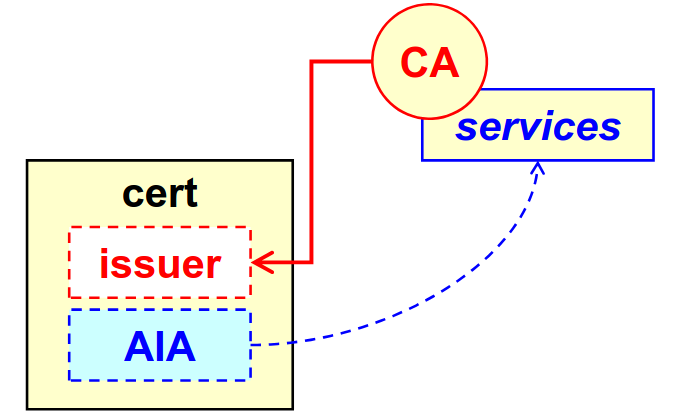
\includegraphics[width=0.5\textwidth]{img/x509 AIA.png}

  \caption{Authority Information Access (AIA) extension}
\end{figure}

\subsubsection{CA Information Access}

The \textbf{CA Information Access (CAIA)} extension serves a 
specific function in X.509 certificates, as it indicates how to 
access information and services provided by the certificate 
authority (CA) that owns the certificate. Unlike other 
extensions, CAIA is valid only within a CA certificate itself.

CAIA includes several important subfields that facilitate access 
to the CA's services, such as:
\begin{itemize}
  \item \textbf{certStatus}: This subfield may point to the status of 
    the CA's certificates, typically through an OCSP responder.
  \item \textbf{certRetrieval}: This allows for the retrieval of the 
    CA's own certificate from a designated location.
  \item \textbf{cAPolicy}: This subfield provides information on the 
    policies that govern the CA's operations, helping users 
    understand the trust model.
  \item \textbf{caCerts}: It indicates where the CA's certificates can 
    be accessed, which is vital for validating the certificate 
    chain.
\end{itemize}

The significance of CAIA lies in its role as a self-pointer for 
the CA. When you possess a CA certificate and wish to locate its 
services, CAIA provides the necessary pointers to information 
about the CA itself, including its policy, OCSP responder, and 
certificate repository. This self-referential nature distinguishes 
CAIA from other access methods, which typically point back to the 
parent CA. As with many extensions, CAIA can be classified as 
either critical or non-critical, depending on the context in 
which it is used. However, it is particularly valuable for 
establishing a complete understanding of the CA's services and 
trustworthiness.

\begin{figure}[h]
  \centering
  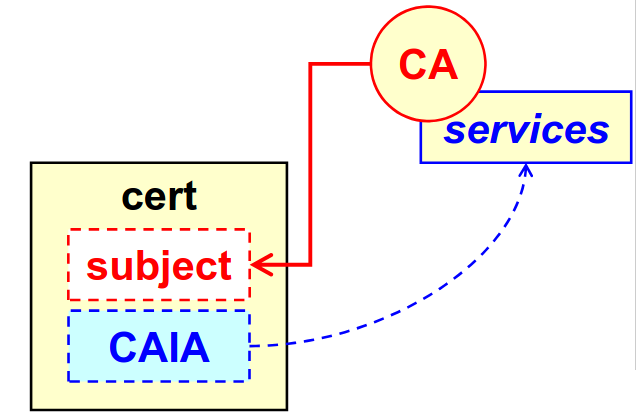
\includegraphics[width=0.5\textwidth]{img/x509 CAIA.png}

  \caption{CA Information Access (CAIA) extension}
\end{figure}

\subsubsection{RFC-2459}

The \textbf{RFC-2459} document defines a profile for the use of 
X.509v3 certificates in Internet applications, such as IPsec, TLS, 
and S/MIME. This profile was initially suggested by the Public Key 
Infrastructure (PKIX) working group to promote interoperability 
and standardization across diverse systems and protocols.

One of the key aspects of RFC-2459 is that it establishes extensions 
defined by an Object Identifier (OID), specifically using the base 
\texttt{ID-PKIX ::= 1.3.6.1.5.5.7} (which maps to 
\texttt{iso.org.dod.inet.sec.mechanisms.pkix}). OIDs ensure that 
each extension and algorithm used within the X.509 framework is 
uniquely identifiable and properly managed. For instance, PKIX 
requested an OID rooted in the U.S. Department of Defense namespace 
due to the historical origin of the internet (as DARPA Net), and 
further sub-trees were established for protocols like IPsec, TLS, 
and S/MIME.

RFC-2459 also specifies the supported algorithms that should be 
implemented to ensure secure and reliable communication. Beyond 
defining supported algorithms, it offers several implementation 
suggestions to enhance compatibility. A few examples include:
\begin{itemize}
    \item \textbf{UTC Time}: It is mandatory to include seconds 
    in time fields.
    \item \textbf{Zulu Time}: UTC time must be expressed in the 
    Zulu (Greenwich Mean Time) timezone, which avoids issues with 
    software systems that misinterpret time zones. For instance, 
    some software (notably from Microsoft) might default to local 
    time, causing inconsistencies.
    \item \textbf{Two-Digit Year Format}: Although specifying the 
    year in two digits is not recommended, when used, it should be 
    interpreted within the range of 1950-2049. After 2049, 
    certificates must switch to four-digit year formats to avoid 
    ambiguity and incompatibility issues.
\end{itemize}

By adhering to the guidelines outlined in RFC-2459, certificate 
issuers and consumers ensure proper functionality across diverse 
systems, especially in the context of internet security protocols. 
The use of standardized extensions, supported algorithms, and 
implementation details like time format further strengthens 
interoperability and the reliability of X.509 certificates.

\subsubsection{Extended Key Usage}

The \textbf{Extended Key Usage} (EKU) extension in X.509 certificates 
allows for defining specific uses of a certificate in addition to, 
or in substitution of, the standard \texttt{keyUsage} extension. 
Unlike the standard key usage, which is focused on cryptographic 
operations, EKU is oriented towards specific applications. This 
enables a certificate to be more narrowly defined for its intended 
purpose, enhancing security and clarity in certificate handling.

EKU can be used simultaneously with the standard \texttt{keyUsage} 
extension, though it is important to consider how conflicts between 
the two might be handled in practice. EKU serves to tailor 
certificates for specific tasks within certain application domains, 
which is particularly useful in environments requiring strict 
certification boundaries, such as server authentication or 
email protection.

Some of the possible values for EKU include:
\begin{itemize}
    \item \texttt{serverAuth} (\texttt{id-pkix.3.1}): This EKU 
    designates a certificate for server authentication. In cases 
    where serverAuth is used, the equivalent key usages that should 
    be enabled include Digital Signature (DS), Key Encipherment (KE), 
    and Key Agreement (KA).
    \item \texttt{clientAuth} (\texttt{id-pkix.3.2}): This EKU is 
    intended for client-side authentication and can be mapped to 
    Digital Signature (DS) and Key Agreement (KA).
    \item \texttt{codeSigning} (\texttt{id-pkix.3.3}): This EKU is 
    used for code signing, allowing developers to sign the code they 
    create. The primary associated key usage is Digital Signature 
    (DS).
    \item \texttt{emailProtection} (\texttt{id-pkix.3.4}): This EKU 
    provides a certificate for email protection. It includes Digital 
    Signature (DS), Non-Repudiation (NR), Key Encipherment (KE), and 
    Key Agreement (KA) as the relevant key usages.
    \item \texttt{timeStamping} (\texttt{id-pkix.3.8}): Used for 
    timestamping, this EKU is associated with Digital Signature (DS) 
    and Non-Repudiation (NR). Timestamping certificates are crucial 
    for certifying when a particular action, such as a signature, 
    took place.
    \item \texttt{ocspSigning} (\texttt{id-pkix.3.9}): This EKU is 
    specific to signing OCSP responses. The associated key usages 
    are Digital Signature (DS) and Non-Repudiation (NR), ensuring 
    that OCSP responses are properly authenticated.
\end{itemize}

In summary, the PKIX group developed EKU to provide more granular 
control over certificate usage within specific applications. For 
example, a certificate intended for email may only be valid for email 
protection, while another for server authentication may only serve 
that purpose. The flexibility offered by EKU allows for more precise 
security policies, tailored to the needs of individual systems or 
applications.

\subsubsection{Evolution of RFC-2459}

The evolution of \textbf{RFC-2459}, which initially defined the 
profile of X.509v3 certificates for use in Internet applications, 
reflects a series of updates and refinements to both certificate 
profiles and cryptographic algorithms.

RFC-2459 was replaced by two key documents:
\begin{itemize}
    \item \textbf{RFC-3280}: This document defines the Internet 
    profile of public key infrastructures (PKIs) based on X.509v3 
    certificates and X.509v2 certificate revocation lists (CRLs). 
    It was intended to standardize how certificates and CRLs are 
    managed and used in Internet-based PKI systems.
    \item \textbf{RFC-3279}: This document covers the algorithms 
    used in conjunction with the RFC-3280 profile, providing 
    identifiers, parameters, and encodings. It includes, and makes 
    obsolete, the earlier RFC-2528, which addressed the use of 
    the Key Exchange Algorithm (KEA).
\end{itemize}

The decision to split RFC-2459 into two separate RFCs was driven by 
the recognition that while certificate profiles tend to remain stable 
over time, cryptographic algorithms evolve more rapidly. By 
documenting algorithms separately in RFC-3279, it became easier to 
update the list of supported algorithms without needing to revise the 
entire certificate profile.

Later on, \textbf{RFC-3280} was itself obsoleted by \textbf{RFC-5280}, 
which further refined the Internet PKI profile and introduced updates 
to align with advancements in cryptographic practices and PKI 
implementation. RFC-5280 remains a foundational document in the 
definition of PKI systems used for securing Internet communication.
\subsubsection{RFC-3279 and Supported Algorithms}

\textbf{RFC-3279} specifies the algorithms that \emph{MUST} be 
supported by applications using the \textbf{RFC-3280} profile. 
It includes some older algorithms, as well as newer ones. The key 
algorithms defined in this RFC are:

\begin{itemize}
  \item \textbf{Digest algorithms:}
  \begin{itemize}
    \item MD-2, MD-5, SHA-1 (preferred)
  \end{itemize}
  \item \textbf{Algorithms for signing certificates/CRLs:}
  \begin{itemize}
    \item RSA, DSA, \underline{ECDSA (Elliptic Curve DSA)}
  \end{itemize}
  \item \textbf{Subject public key algorithms (SubjectPublicKeyInfo):}
  \begin{itemize}
    \item RSA, DSA, \underline{KEA}(a variant of Diffie-Hellman), DH
      (Diffie-Hellman), \underline{ECDSA}, \underline{ECDH (Elliptic
      Curve Diffie-Hellman)}
  \end{itemize}
\end{itemize}

The underlined algorithms were introduced in \textbf{RFC-3279} in 
comparison to \textbf{RFC-2459}. One important point is that RFC-3279 
permits the use of legacy algorithms, though they are not recommended 
(e.g., SHA-1 is preferred for digest, and RSA/DSA for certificate 
signing, with ECDSA added for more modern use). 

Once the basic definitions are set, optional algorithms can be defined. 
Notably:

\begin{itemize}
  \item \textbf{RFC-4055:} Adds better specifications for signatures, 
    including the Probabilistic Signature Scheme (PSS), Optimal 
    Asymmetric Encryption Padding (OAEP), and SHA-2 for digest 
    computation.
  \item \textbf{RFC-4491:} Addresses the needs of Russia by providing 
    specifications for the \emph{GOST} algorithm family, widely used 
    in Russian encryption standards.
  \item \textbf{RFC-5480:} Introduces elliptic curve keys of various 
    kinds.
  \item \textbf{RFC-5758:} Adds support for new algorithms in the 
    \emph{SHA-2} family, such as SHA-224 and SHA-256.
  \item \textbf{RFC-8692:} Uses SHAKE128 and SHAKE256 for signatures, 
    both part of the \emph{SHA-3} family of algorithms.
\end{itemize}

\subsubsection{RFC-3280 / RFC-5280: PKI Profile}

\textbf{RFC-3280} and \textbf{RFC-5280} specify the profile that defines 
not only values and fields but also algorithms and procedures. These 
ensure that certificates are processed consistently across the world. 
Key aspects include:

\begin{itemize}
  \item \textbf{Path validation algorithm:} Defines how to build or 
    verify the certificate chain, starting from an end entity (EE) 
    certificate, which is issued by a CA, up to a trusted root.
  \item \textbf{Certificate status verification:} Specifies details 
    for verifying the status of a certificate, using methods such as 
    the full CRL or Delta-CRL.
  \item \textbf{Extended Key Usage (EKU):} Adds the \emph{OCSPSigning} 
    extended key usage.
  \item \textbf{Certificate extensions:} Includes important extensions 
    such as:
  \begin{itemize}
    \item \textbf{Inhibit any-policy:} Prevents the use of any policy, 
      ensuring that the CA must specify its own policies.
    \item \textbf{Freshest CRL:} A pointer to a new type of CRL 
      (Delta-CRL), which contains only the differences with the last 
      full CRL.
    \item \textbf{Subject information access:} Already discussed 
      previously.
  \end{itemize}
  \item \textbf{Freshest CRL for CRLs:} If there is a Delta-CRL 
    pointer in a certificate or CRL, it is possible to access the 
    differences with the last full CRL. The Freshest CRL is also known 
    as the Delta CRL Distribution Point. It is always marked as 
    non-critical because there are multiple ways to check certificate 
    status (e.g., full CRL, Delta CRL, OCSP), and it is not feasible 
    to make any single method mandatory.
\end{itemize}

\subsubsection{Additional Points}

\begin{itemize}
  \item \textbf{Path validation focus:} Due to the sensitive nature of 
    path validation, recent RFCs have paid much more attention to 
    specifying the algorithms for this process, rather than just 
    providing high-level descriptions as in earlier versions. 
  \item \textbf{Support for internationalization:} With global use of 
    certificates, it has become important to support different 
    alphabets, such as those used in Japan, China, and India, in 
    fields like URI, DNS names, and email addresses. \textbf{RFC-8398} 
    adds support for internationalized email addresses and domain 
    names.
  \item \textbf{Freshest CRL pointer:} A crucial feature is the 
    \emph{Freshest CRL} pointer, which allows a certificate or CRL to 
    reference the latest Delta-CRL. This prevents the need to 
    redownload a full CRL when only small updates are necessary.
  \item \textbf{No Delta of Delta-CRLs:} Delta CRLs cannot be created 
    incrementally (i.e., you cannot generate a Delta of a Delta CRL). 
    Each Delta CRL must reference the base CRL directly, making the 
    process more straightforward.
\end{itemize}

